\chapter{EL SURGIMIENTO DEL SERIALISMO INTEGRAL}
	\section{Alban Berg y Anton Webern: la Segunda Escuela de Viena}
	\label{berweb}
	Además de Schoenberg, hubo dos compositores más que contribuyeron al desarrollo del dodecafonismo y que demostraron con sus diferentes estilos la versatilidad del sistema. Éstos fueron los discípulos de Schoenberg: Alban Berg y Anton Webern. 
	
	El maestro y sus dos alumnos formaron la autodenominada Segunda Escuela de Viena, llamada así en honor a los miembros de la Primera Escuela de Viena: Haydn, Mozart y Beethoven. Aparte del hecho de que Schoenberg, Berg y Webern nacieron y se formaron en Viena, el nombre también simboliza su autoproclamación como herederos legítimos de la tradición musical alemana proveniente del siglo XVIII.
	
	La Segunda Escuela de Viena formó parte de las vanguardias artísticas europeas, opuestas a la tendencia neoclásica de Stravinsky o Prokofiev. Los tres integrantes siguieron carreras compositivas similares en cuanto a estilo y concepción artística: una época tonal, una ruptura atonal y un desarrollo dodecafónico.
	
	Con el ascenso del nazismo, Schoenberg, que era judío, se vio obligado a exiliarse a Estados Unidos. Sus discípulos se quedaron en Austria, pero pasaron penurias económicas debido a la censura impuesta por el gobierno: la música dodecafónica se descalificó como \emph{Entartete Musik} (<<música degenerada>>).
	
	\begin{wrapfigure}{L}{0.3\textwidth}
		\captionsetup{justification=centering, font=footnotesize}
		\vspace{0cm}
		\centering{
			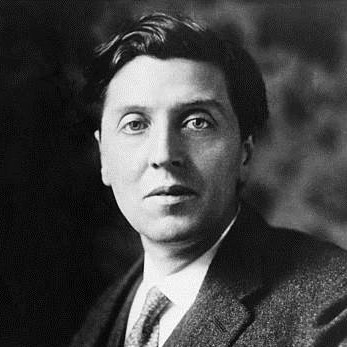
\includegraphics[width=0.22\textwidth]{Alban_Berg.jpg}			
			\caption*{Alban Berg\\(1885--1935)}	}
	\end{wrapfigure}
	Alban Berg se centró en la efusión emocional y el interés por lo humano, utilizando el método dodecafónico libremente y acercándose a formatos tonales. Su etapa atonal fue especialmente relevante, ya que compuso entonces su primera obra dramática, Wozzeck (1925). Es una ópera basada en la pieza teatral de Georg Büchner, en la cual Berg plasmó parte de sus propias experiencias como soldado en la Primera Guerra Mundial. Su segunda ópera, Lulú, quedó inconclusa debido a su muerte por septicemia en 1935, a los 50 años.
	
	Anton Webern fue un compositor más riguroso en cuanto a las formas, siempre leal al sistema dodecafónico y a su maestro. Se deleitaba en los procedimientos formales más sutiles, aquellos que solo podían ser descubiertos al estudiar detenidamente la obra. Esto quedó reflejado en su dodecafónico Concierto para 9 instrumentos, Op. 24 (1934), cuya serie está construida por segmentos derivados de las tres primeras notas de la obra. Además, muestra tendencias a asignar duraciones, timbres y articulaciones a segmentos aislados, lo que más tarde inspiraría el serialismo integral.
        
	Durante la ocupación de Viena, Webern salió de su casa una noche tras el toque de queda, y un soldado norteamericano, probablemente en estado de embriaguez, lo mató a tiros. Así, Schoenberg, el maestro y el más mayor de los tres, sobrevivió a sus dos alumnos exiliado en Estados Unidos.
    
	\section{La escuela de Darmstadt}
	Tras la Segunda Guerra Mundial, el mundo artístico estaba totalmente destruido. La violencia, la censura y la incomunicación habían impedido cualquier posible desarrollo creativo, y los artistas de la generación anterior se habían aislado, exiliado o habían fallecido. Volver a construir los pilares del arte era el cometido de la nueva generación de artistas, quienes compartían la sensación de que el mundo había renacido y el tiempo había comenzado de nuevo.
	
	En 1946 se fundaron los Cursos de Verano de Darmstadt, fundados por Wolfgang Steinecke y patrocinados por las fuerzas americanas, con el objetivo de retomar la actividad musical en la Alemania de la posguerra. Los cursos se centraron en dar a conocer las técnicas compositivas de las generaciones anteriores. Aunque el primer año estuvo enfocado en el movimiento neoclásico, fue en los años posteriores cuando se desarrolló un mayor interés por las técnicas serialistas.
	
	Los cursos resultaron en la aparición de una nueva escuela de compositores cuya finalidad artística era crear un lenguaje musical distinto y alejado de la tradición para, de esta forma, obtener una mayor libertad compositiva. Esta escuela tomó el nombre de la ciudad donde se realizaban los cursos: se llamó la Escuela de Darmstadt. El término fue acuñado por el compositor Luigi Nono en una de sus clases magistrales en 1957, y con él se describía a sí mismo y a sus compañeros compositores: Pierre Boulez, Karlheinz Stockhausen y Bruno Maderna. Para estos compositores, la tradición artística estaba demasiado relacionada con los fracasos políticos y las penurias sociales pasadas, y precisamente por ello creían necesario romper con todos los vínculos heredados.
	
	\begin{wrapfigure}{R}{0.3\textwidth}
		\captionsetup{justification=centering, font=footnotesize}
		\vspace{-0.5cm}
		\centering{
			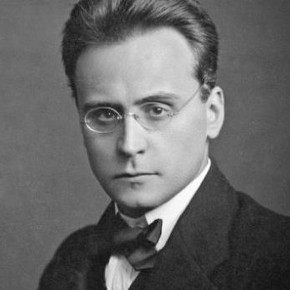
\includegraphics[width=0.22\textwidth]{Anton_Webern.jpg}			
			\caption*{Anton Webern\\(1883--1945)}	}
	\end{wrapfigure}
    Sin embargo, para crear aquel nuevo lenguaje no tomaron como referencia el dodecafonismo de Schoenberg, ya que él veía su sistema como parte de la tradición musical, como un elemento más en la evolución de la música. Se centraron, en cambio, en la formalidad y abstracción del serialismo de Anton Webern, y desarrollaron a partir de sus métodos el denominado \emph{serialismo integral}. Para la Escuela de Viena, el estilo compositivo de Webern era tan solo un posible enfoque del amplio abanico que abarcaba el dodecafonismo, pero la Escuela de Darmstadt lo consideró como un avance de éste.
	
	El serialismo integral es un sistema de composición musical que predetermina los materiales compositivos -- la melodía, la armonía, el ritmo, el timbre -- a partir de la ordenación serial de los diferentes parámetros musicales: alturas, intensidades, duraciones, ataques o instrumentos, entre otros. Es un desarrollo del serialismo dodecafónico de Schoenberg, que serializa solamente las alturas, hacia los demás parámetros sonoros. Tiene, por tanto, un alto grado de planificación pre-composicional: se pretende que la determinación compositiva sea absoluta; y se tiende al automatismo del arte y sus formas, alejándolo de cualquier evocación decimonónica.

	Desde sus comienzos, el serialismo integral suscitó numerosas críticas, incluso desde el propio colectivo vanguardista. Una de ellas fue la falta de elección del intérprete a la hora de transmitir la obra. El intérprete serialista debe reproducir con total exactitud cada detalle de la partitura, y, por tanto, no puede aportar carácter alguno. Otra de las críticas más extendidas fue la incapacidad para interpretar estas obras correctamente debido a su complejidad técnica. Además, los detalles que precisamente las hacen complejas son, en su mayor parte, inapreciables por parte del oyente.

	\section{Pierre Boulez}
	\label{boulez}
     \begin{wrapfigure}{L}{0.3\textwidth}
		\captionsetup{justification=centering, font=footnotesize}
		\vspace{-0.5cm}
		\centering{
			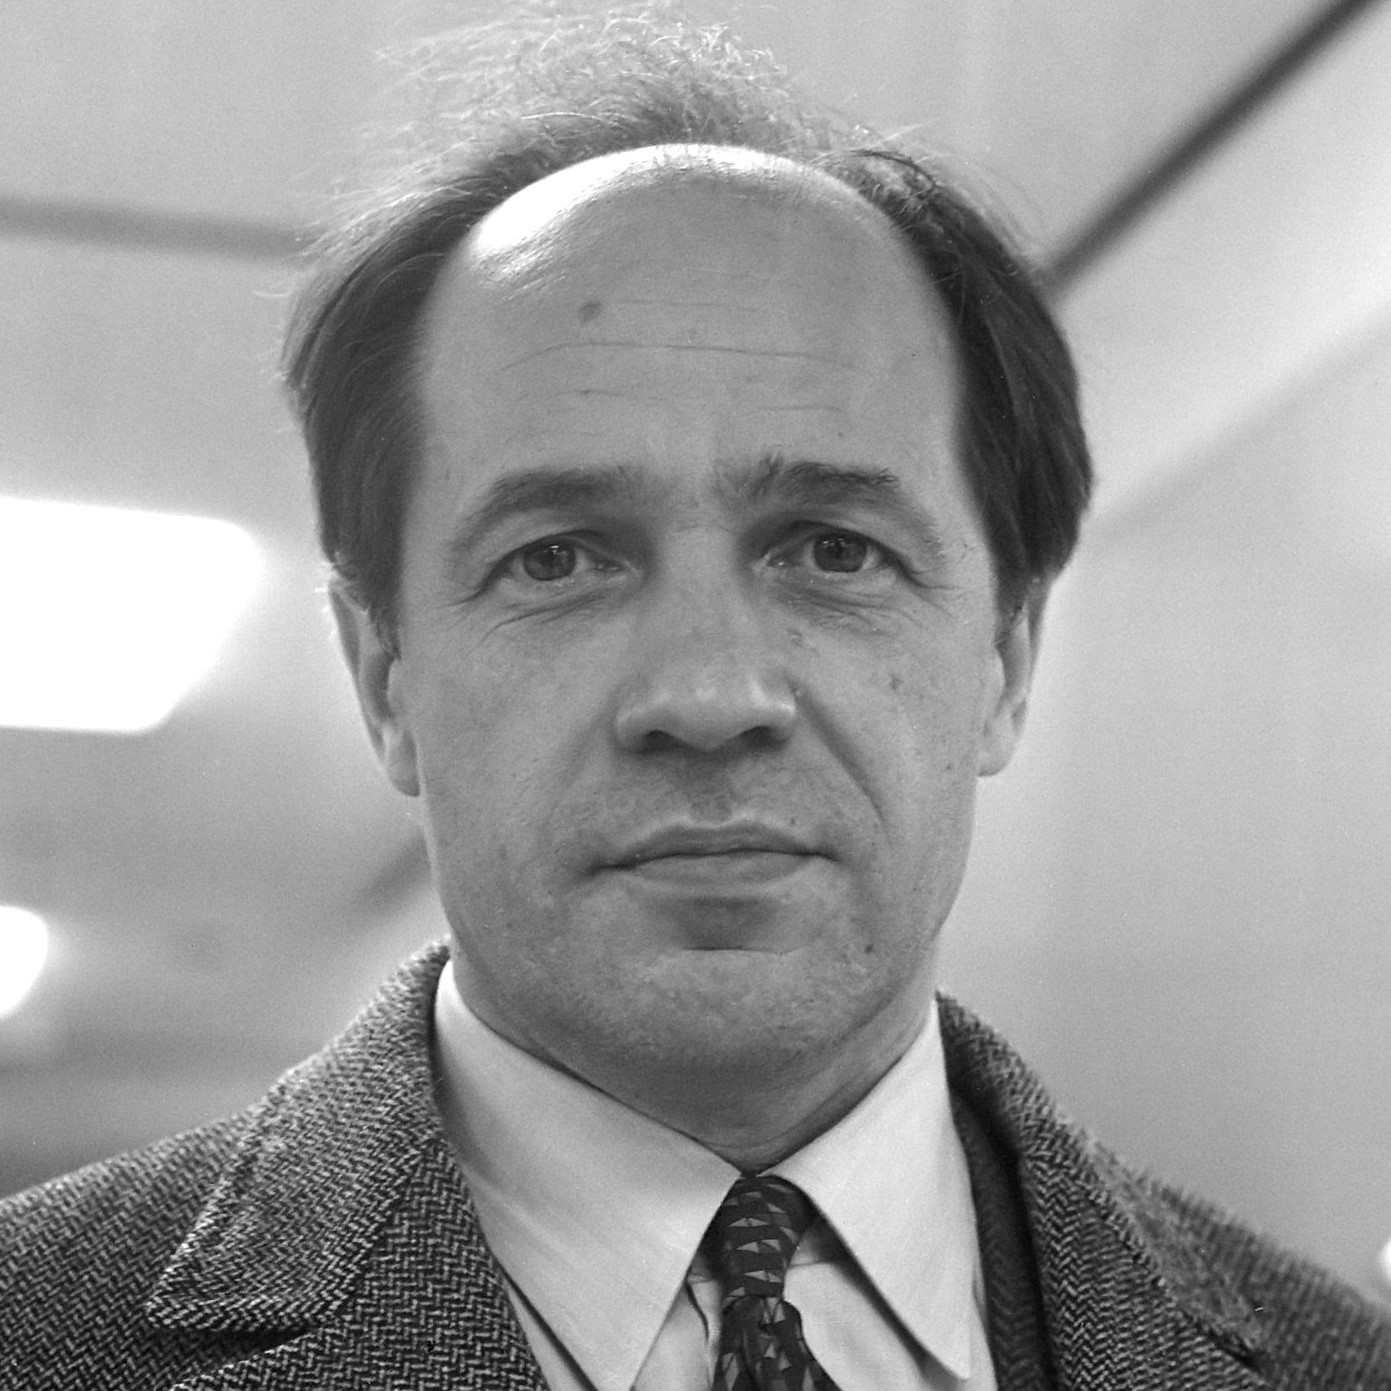
\includegraphics[width=0.22\textwidth]{Pierre_Boulez.jpg}			
			\caption*{Pierre Boulez\\(1925--2016)}	}
	\end{wrapfigure}
    El compositor que creó y utilizó por primera vez el serialismo integral, además de instruirlo y difundirlo a los demás compositores de Darmstadt, fue el compositor francés Pierre Boulez. Otros músicos habían compuesto obras con tendencias serialistas y elementos predeterminados, como Olivier Messiaen en \emph{Mode de valeurs et d’intensités}, pero fue Boulez quien sentó sus bases y su técnica. De hecho, los compositores precedentes influyeron prominentemente en la música de Boulez gracias a las clases impartidas en los cursos de Darmstadt.
    
    Boulez consideraba necesaria y evidente la extensión de elementos a predeterminar más allá de la melodía, y le parecía incoherente el sistema dodecafónico de Schoenberg, que para él estaba incompleto. En su controvertido ensayo \emph{Schoenberg ha muerto}, publicado un año después de la muerte del compositor, comentó:
    
    \begin{quote}\emph{En primer lugar, la exploración del campo serial ha sido conducida unilateralmente: allí falta el plano rítmico, e incluso el plano sonoro propiamente dicho: las intensidades y los ataques.} [$\ldots$] \emph{Pero la causa esencial de su fracaso reside en el desconocimiento profundo de las FUNCIONES seriales propiamente dichas, las funciones engendradas por el principio mismo de la serie.}\footnote{Pierre Boulez, \emph{Schoenberg is dead}, en la revista \emph{The Score}, 1952.}\end{quote}
    
   Es decir, que para ampliar el concepto de serialismo se debía primeramente conocer el fundamento matemático de las series y sus funciones transformativas. Además de ser músico y compositor, Boulez había estudiado matemáticas, lo que le llevó a querer analizar matemáticamente el sistema compositivo y generalizarlo para series de longitudes arbitrarias. Para él, el serialismo no debía ser un mero recurso compositivo, sino la ley que rige todos los elementos de la obra. De hecho, más adelante en su ensayo declara:
    
    \begin{quote}[\ldots] \emph{desde el descubrimiento de la Escuela de Viena, todo compositor alejado de los experimentos seriales ha resultado inútil.}\end{quote}

	Su obra \emph{Structures I} (1952), para dos pianos, fue compuesta siguiendo las técnicas de serialismo integral: tiene series de doce alturas, doce ataques, doce duraciones y
doce tipos dinámicos, aunque más tarde reduciría algunas a diez.